% BHU PYQ -- Professional Exam Template
\documentclass[11pt,a4paper]{article}

\usepackage[a4paper,top=2.5cm,bottom=2.5cm,left=2.8cm,right=2.8cm,headheight=14pt]{geometry}
\usepackage{amsmath,amssymb}
\usepackage[T1]{fontenc}
\usepackage[utf8]{inputenc}
\usepackage{lmodern}
\usepackage{microtype}
\usepackage{fancyhdr}
\usepackage{enumitem}
\usepackage{hyperref}
\usepackage{lastpage}
\usepackage{parskip}
\usepackage{tikz}
\usetikzlibrary{arrows.meta,shapes,positioning}

\hypersetup{colorlinks=true,urlcolor=black,linkcolor=black,
  pdftitle={B.Sc. (Hons.) Zoology Sem-V ZOB-505 -- BHU PYQ}}

\pagestyle{fancy}
\fancyhf{}
\renewcommand{\headrulewidth}{0.4pt}
\renewcommand{\footrulewidth}{0.4pt}
\fancyhead[L]{\small   \textit{Banaras Hindu University}}
\fancyhead[R]{\small   \textit{Zoology Paper: ZOB-505}}
\fancyfoot[C]{\small Page  \thepage\ of \pageref{LastPage}}


\newlist{parts}{enumerate}{2}
\setlist[parts,1]{label=(\alph*),leftmargin=*,itemsep=4pt,topsep=3pt}
\setlist[parts,2]{label=(\roman*),leftmargin=*,itemsep=2pt,topsep=2pt}

\newcommand{\pts}[1]{\hfill   \textit{[#1]}}


\begin{document}


\begin{center}
  {\large\bfseries BANARAS HINDU UNIVERSITY}\\[2pt]
  {\normalsize B.Sc. (Hons.) Semester V Examination, 2022-23}\\[6pt]
  \rule{0.8\linewidth}{0.5pt}\\[6pt]
  {\large\bfseries Zoology}\\[4pt]
  {\large\bfseries Paper: ZOB-505 --- Environmental Biology and Systematics}\\[4pt]
  {\normalsize Time: Three hours \hfill Full Marks: 70}
\end{center}

\rule{\linewidth}{0.4pt}

\smallskip



\noindent   \textit{Note: Answer four questions from Section-A (including Question No. 1 which is compulsory) and three questions from Section-B (including Question No. 1 which is compulsory). Use a separate answer book for each section. The figures in the right-hand margin indicate marks.}

\bigskip

\begin{center}
   \textbf{SECTION -- A} \\
   \textbf{(Environmental Biology) (Marks: 45)}
\end{center}

\medskip


\noindent   \textbf{Question 1.} Answer the following parts:

\begin{parts}
  \item Write whether the following statements are True or False. Justify your answer in 2-3 sentences each:\pts{$2  \times 5 = 10$}
  
\begin{parts}
    \item The oceans are biological deserts.
    \item The transport of oxygen from lungs to other parts of the body is facilitated by carboxyhaemoglobin.
    \item Stratospheric ozone forms naturally and helps shield us from ultraviolet radiation of sunlight.
    \item Hexavalent chromium is not a pollutant and is beneficial to humans.
    \item Invasive exotic species are the main threat to biodiversity.
  \end{parts}
  
  \item Define the following terms:\pts{$1  \times 5 = 5$}
  
\begin{parts}
    \item Keystone species
    \item Gross primary productivity
    \item Ecesis
    \item Fecundity rate
    \item Pyramid of energy
  \end{parts}
\end{parts}

\medskip


\noindent   \textbf{Question 2.} Write an essay on the aquatic ecosystems.\pts{10}

\medskip


\noindent   \textbf{Question 3.} What is solid waste pollution? Describe various methods of solid waste management along with their advantages.\pts{10}

\medskip


\noindent   \textbf{Question 4.} Write an essay on the nature, structure, and attributes of a biological community.\pts{10}

\medskip


\noindent   \textbf{Question 5.} Write short notes on the following:\pts{$2.5  \times 4 = 10$}

\begin{parts}
  \item Food web
  \item Energy flow in ecosystem
  \item Positive interactions
  \item Biodiversity conservation
\end{parts}

\pagebreak

\begin{center}
   \textbf{SECTION -- B} \\
   \textbf{(Systematics) (Marks: 25)}
\end{center}

\medskip


\noindent   \textbf{Question 1.} Answer the following parts:

\begin{parts}
  \item Write whether the following statements are True or False. Justify your answer in 2-3 sentences each:\pts{$2  \times 2 = 4$}
  
\begin{parts}
    \item Tribe is a lower taxonomic category that comes between genus and species.
    \item DNA-DNA hybridization is a more reliable method to establish genetic similarity between two species than comparing their nucleotide sequences of certain common genes.
  \end{parts}
  
  \item Define the following terms:\pts{$1  \times 3 = 3$}
  
\begin{parts}
    \item Taxon
    \item Tautonym
    \item Binomial nomenclature
  \end{parts}
\end{parts}

\medskip


\noindent   \textbf{Question 2.} Discuss the following:\pts{$4.5  \times 2 = 9$}

\begin{parts}
  \item Molecular taxonomy
  \item Taxonomic characters
\end{parts}

\medskip


\noindent   \textbf{Question 3.} What is a species? Discuss different types of species concepts and specify which one of the concepts finds maximum acceptance from biologists, giving the reasons for its acceptance.\pts{9}

\medskip


\noindent   \textbf{Question 4.} Write notes on the following:\pts{$1.5  \times 6 = 9$}

\begin{parts}
  \item DNA barcoding
  \item Polytypic species
  \item Phylogenetic tree
  
  
\begin{center}
  
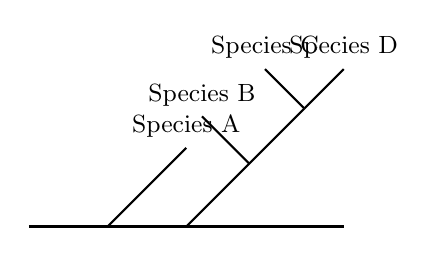
\begin{tikzpicture}[scale=1.0, >=Stealth, every node/.style={font=\small}]
    \draw[thick] (0,0) -- (4,0);
    \draw[thick] (1,0) -- (2,1) node[above] {Species A};
    \draw[thick] (2,0) -- (3.5,1.5);
    \draw[thick] (2.8,0.8) -- (2.2,1.4) node[above] {Species B};
    \draw[thick] (3.5,1.5) -- (3,2) node[above] {Species C};
    \draw[thick] (3.5,1.5) -- (4,2) node[above] {Species D};
    
ode[below] at (2,0) {Common Ancestor};
  \end{tikzpicture}
  \end{center}

  \item Alpha taxonomy
  \item Genus
  \item Category
\end{parts}

\vfill
\rule{\linewidth}{0.4pt}

\begin{center}\small
\href{https://bhu-exam.vercel.app/}{Click Here}\\[4pt]\href{https://me-aryan.vercel.app/}{Click Here}\\[4pt]\href{https://quashan-me.vercel.app/}{Click Here}
\end{center}

\end{document}
